\documentclass{exam}
\usepackage{graphicx}
\usepackage[utf8]{inputenc}
\usepackage[english]{babel}
\usepackage{amsmath}
\usepackage{hyperref}
\usepackage{amsthm}
\usepackage{tcolorbox}
\usepackage{amsfonts}
\usepackage{amssymb}
\usepackage{mathrsfs}
\usepackage{centernot}

\newcommand{\paren}[1]{\left(#1\right)}

\allowdisplaybreaks

\makeatletter
\long\def\paragraph{%
  \@startsection{paragraph}{4}%
  {\z@}{2ex \@plus 1ex \@minus .2ex}{-1em}%
  {\normalfont\normalsize\bfseries}%
}
\makeatother

\DeclareMathOperator{\lcm}{lcm}

\newbox\eeveebox
\setbox\eeveebox\hbox{
\raisebox{-2.5pt}{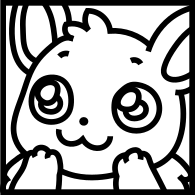
\includegraphics[height=2.5ex]{iibui.png}}}
\def\eeveeKawaii{\copy\eeveebox}

\newbox\skullbox
\setbox\skullbox\hbox{
\raisebox{-2.5pt}{
\includegraphics[height=2.5ex]{skull.png}}}
\def\bendingskull{\copy\skullbox}

\NewTColorBox{proposition}{m}{
  standard jigsaw,
  sharp corners,
  boxrule=0.4pt,
  coltitle=black,
  colframe=black,
  opacityback=0,
  opacitybacktitle=0,
  fonttitle=\normalfont\bfseries\upshape,
  fontupper=\normalfont\itshape,
  title={Proposition #1},
  after title={.},
  attach title to upper={\ },
}

\NewTColorBox{theorem}{m}{
  standard jigsaw,
  sharp corners,
  boxrule=0.4pt,
  coltitle=black,
  colframe=black,
  opacityback=0,
  opacitybacktitle=0,
  fonttitle=\normalfont\bfseries\upshape,
  fontupper=\normalfont\itshape,
  title={Theorem #1},
  after title={.},
  attach title to upper={\ },
}

\renewcommand\qedsymbol{$\eeveeKawaii$}

\title{Hammack Exercises - Chapter 10}
\author{FungusDesu}
\date{September 21th 2024}

\begin{document}

\maketitle

\section{Preface}
i dont really have anything to say

\section{Induction}

\begin{proposition}{10.1}
    $$1+2+3+4+\dots+n=\frac{n^2+n}2$$ for some positive integer n.
\end{proposition}

\begin{proof}
    Denote $S_n: 1 + 2 + 3 + \dots + n=\frac{n^2+n}{2}$. We will prove this using induction. 
    \paragraph{Basis step.} If $n= 1$, then the equation is true.
    \paragraph{Inductive hypothesis.} For $k\ge 1$, suppose $S_k$ is true; that is, $1 + 2 + 3 +\dots + k = \frac{k^2+k}2$. We wish to prove $S_{k+1}$ is true.
    \paragraph{Induction step.} Observe that:
    \begin{align*}
        1 + 2 + 3 +\dots + k + 1 &= 1 + 2 + 3 + \dots + k + k + 1\\
        &=\frac{k^2 + k}2 + k + 1\\
        &=\frac{k^2 + 3k + 2}{2}\\
        &=\frac{(k+1)^2+(k+1)}2.
    \end{align*}
    Thus $1 + 2 + 3 +\dots + k + 1 = \frac{(k+1)^2+(k+1)}2$, which implies $S_k\implies S_{k+1}$. This completes our proof.
\end{proof}

\begin{proposition}{10.2}
    $$1^2+2^2+3^2+4^2+\dots+n^2=\frac{n(n+1)(2n+1)}6$$ for every positive integer $n$.
\end{proposition}

\begin{proof}
    Denote $S_n: 1^2 + 2^2 + \dots + n^2 = \frac{n(n+1)(2n+1)}6$. We will prove this using induction.
    \paragraph{Basis step.} If $n = 1$, then $S_1$ is true.
    \paragraph{Inductive hypothesis.} For $k\ge 1$, suppose $S_k$ is true; that is, $1^2 + 2^2 +\dots+k^2=\frac{k(k+1)(2k+1)}6$. We wish to prove $S_{k+1}$ is true.
    \paragraph{Induction step.} Observe that:
    \begin{align*}
        1^2 + 2^2 +\dots+(k+1)^2 &= 1^2 + 2^2 + \dots + k^2 + (k+1)^2 = \frac{k(k+1)(2k+1)}6 + (k+1)^2\\
        &= \frac{(k+1)(k(2k+1) + 6k+6)}6= \frac{(k+1)(2k^2 + 7k + 6)}{6}\\
        &=\frac{(k+1)(k+2)(2k+3)}6=\frac{(k+1)((k+1)+1)(2(k+1)+1)}6.
    \end{align*}
    Thus $1^2 + 2^2 +\dots+(k+1)^2 =\frac{(k+1)((k+1)+1)(2(k+1)+1)}6$, which implies $S_k\implies S_{k+1}$. This completes our proof.
\end{proof}

\begin{proposition}{10.3}
    $$1^3+2^3+3^3+4^3+\dots+n^3=\frac{n^2(n+1)^2}{4}$$ for every positive integer $n$.
\end{proposition}

\begin{proof}
    Denote $S_n:1^3+2^3+\dots+n^3=\frac{n^2(n+1)^2}4$. We shall prove this by induction.
    \paragraph{Basis step.} If $n =1$, then the equation is true.
    \paragraph{Inductive hypothesis.} For $k\ge 1$, suppose $S_k$ is true; that is, $1^3 + 2^3 +\dots+k^3 = \frac{k^2(k+1)^2}4$. We wish to prove $S_{k+1}$ is true.
    \paragraph{Induction step.} Observe that:
    \begin{align*}
        1^3 + 2^3 +\dots + (k+1)^3 &= 1^3 + 2^3 +\dots + k^3 + (k+1)^3 = \frac{k^2(k+1)^2}4 + (k+1)^3\\
        &=\frac{(k+1)^2(k^2+4k+4)}4=\frac{(k+1)^2(k+2)^2}4\\
        &=\frac{(k+1)^2((k+1)+1)^2}4.
    \end{align*}
    Thus $1^3+2^3+\dots+(k+1)^3=\frac{(k+1)^2((k+1)+1)^2}4$, which implies $S_k\implies S_{k+1}$. This completes our proof.
\end{proof}

\begin{proposition}{10.4}
    If $n\in\mathbb N$, then $$1\cdot2+2\cdot3+3\cdot4+4\cdot5+\dots+n(n+1)=\frac{n(n+1)(n+2)}3.$$
\end{proposition}

\begin{proof}
    Denote $S_n:1\cdot2+2\cdot3+\dots+n(n+1)=\frac{n(n+1)(n+2)}3$. We will prove this using induction.
    \paragraph{Basis step.} If $n=1$, then the equation is true.
    \paragraph{Inductive hypothesis.} For $k\ge 1$, suppose $S_k$ is true; that is, $1\cdot2+2\cdot3+\dots+k(k+1)=\frac{k(k+1)(k+2)}3$. We wish to prove $S_{k+1}$ is true.
    \paragraph{Induction step.} Observe that:
    \begin{align*}
        1\cdot2+2\cdot 3+\dots+(k+1)(k+2) &= 1\cdot2 + 2\cdot3 + \dots + k(k+1) + (k+1)(k+2)\\
        &= \frac{k(k+1)(k+2)}3+(k+1)(k+2)\\
        &=\frac{(k+1)(k+2)(k+3)}3\\
        &=\frac{(k+1)((k+1)+1)((k+1)+2)}3.
    \end{align*}
    Thus $1\cdot2+2\cdot 3+\dots+(k+1)(k+2)=\frac{(k+1)((k+1)+1)((k+1)+2)}3$, which implies $S_k\implies S_{k+1}$. This completes our proof.
\end{proof}

\begin{proposition}{10.5}
    If $n\in\mathbb N$, then $$2^1+2^2+2^3+\dots+2^n=2^{n+1}-2.$$
\end{proposition}

\begin{proof}
    Denote $S_n:2^1+2^2+\dots+2^n=2^{n+1}-2$. We shall prove this using induction.
    \paragraph{Basis step.} If $n = 1$, then the equation is true.
    \paragraph{Inductive hypothesis.} For $k \ge 1$, suppose $S_k$ is true; that is, $2^1+2^2+\dots+2^k=2^{k+1}-2$. We wish to show that $S_{k+1}$ is true.
    \paragraph{Induction step.} Observe that:
    \begin{align*}
        2^1+2^2+\dots+2^{k+1} &= 2^1 + 2^2 +\dots + 2^k + 2^{k+1}\\
        &=2^{k+1}-2+2^{k+1}\\
        &=2^{k+2}-2\\
        &=2^{(k+1)+1}-2.
    \end{align*}
    Thus $2^1+2^2+\dots+2^{k+1}=2^{(k+1)+1}-2$, which implies $S_k\implies S_{k+1}$. This completes our proof.
\end{proof}

\begin{proposition}{10.6}
    $$\sum_{i=1}^n(8i-5)=4n^2-n$$ for every positive integer $n$.
\end{proposition}

\begin{proof}
    Denote the following: $$S_n:\sum_{i=1}^n(8i-5)=4n^2-n.$$ We shall prove this by using induction.
    \paragraph{Basis case.} If $n=1$, then the equation is true.
    \paragraph{Inductive hypothesis.} For $k\ge1$, suppose $S_k$ is true; that is, $$\sum_{i=1}^k(8i-5)=4k^2-k.$$ We wish to prove that $S_{k+1}$ is true.
    \paragraph{Induction step.} Observe the following:
    \begin{align*}
        \sum_{i=1}^{k+1}(8i-5)&=\sum_{i=1}^k(8i-5) + (8(k+1)-5)\\
        &=4k^2-k+8k+8-5\\
        &=4k^2+8k+4-k-1\\
        &=4(k+1)^2-(k+1).
    \end{align*}
    Thus $S_k$ implies $S_{k+1}$. This completes our proof.
\end{proof}

\begin{proposition}{10.7}
    If $n\in\mathbb N$, then $$1\cdot3+2\cdot4+3\cdot5+4\cdot6+\dots+n(n+2)=\frac{n(n+1)(2n+7)}6.$$
\end{proposition}

\begin{proof}
    Denote $S_n:1\cdot3+2\cdot4+\dots+n(n+2)=\frac{n(n+1)(2n+7)}6$. We shall prove this using induction.
    \paragraph{Basis step.} If $n=1$, then the equation is true.
    \paragraph{Inductive hypothesis.} For $k \ge n$, suppose $S_k$ is true; that is, $1\cdot3+2\cdot4+\dots+k(k+2)=\frac{k(k+1)(2k+7)}6$. We wish to prove $S_{k+1}$ is true.
    \paragraph{Induction step.} Observe the following:
    \begin{align*}
        1\cdot3+2\cdot4+\dots+(k+1)(k+3)&=1\cdot3+2\cdot4+\dots+k(k+2)+(k+1)(k+3)\\
        &=\frac{k(k+1)(2k+7)}6+(k+1)(k+3)\\
        &=\frac{(k+1)(2k^2+13k+18)}6\\
        &=\frac{(k+1)(k+2)(2k+9)}6\\
        &=\frac{(k+1)((k+1)+1)(2(k+1)+7)}6.
    \end{align*}
    Thus $S_k$ implies $S_{k+1}$. This completes our proof.
\end{proof}

\begin{proposition}{10.8}
    If $n\in\mathbb N$, then $$\frac1{2!}+\frac2{3!}+\frac3{4!}+\dots+\frac{n}{(n+1)!}=1-\frac{1}{(n+1)!}.$$
\end{proposition}

\begin{proof}
    We shall prove this using induction. Denote $S_n$ to be the following: $$S_n:\frac1{2!}+\frac2{3!}+\dots+\frac{n}{(n+1)!}=1-\frac{1}{(n+1)!}.$$
    \paragraph{Basis step.} The equation holds if $n = 1$.
    \paragraph{Inductive hypothesis.} For $k\ge 1$, suppose $S_k$ is true; that is, $$\frac1{2!}+\frac2{3!}+\dots+\frac{k}{(k+1)!}=1-\frac{1}{(k+1)!}.$$ We wish to prove $S_{k+1}$ is true.
    \paragraph{Induction step.} Observe the following:
    \begin{align*}
        \frac1{2!}+\frac2{3!}+\dots+\frac{k+1}{(k+2)!}&=\frac1{2!}+\frac2{3!}+\dots+\frac{k}{(k+1)!}+\frac{k+1}{(k+2)!}\\
        &=1-\frac1{(k+1)!}+\frac{k+1}{(k+2)!}\\
        &=1-\frac{k+2-k-1}{(k+2)!}\\
        &=1-\frac{1}{((k+1)+1)!}.
    \end{align*}
    Thus $S_k$ implies $S_{k+1}$. This completes our proof.
\end{proof}

\begin{proposition}{10.9}
    $24\mid(5^{2n}-1)$ for every integer $n\ge0$.
\end{proposition}

\begin{proof}
    Denote $S_n:24\mid(5^{2n}-1)$. We shall prove this using induction.
    \paragraph{Basis step.} If $n = 0$, then we have $24\mid0$, which is true.
    \paragraph{Inductive hypothesis.} For $k\ge0$, suppose $S_k$ is true; that is, $24\mid(5^{2k}-1)$. We wish to show that $S_{k+1}$ is true.
    \paragraph{Induction step.} Observe that
    \begin{align*}
        5^{2(k+1)}-1-(5^{2k}-1)&=25^{k+1}-1-25^k+1\\
        &=25\cdot25^k-25^k\\
        &=24\cdot25^k.
    \end{align*}
    We can see that $5^{2(k+1)}-1$ and $5^{2k}-1$ differ by a multiple of 24. Since $24$ divides the latter, $24$ must also divides the former. Thus $S_{k+1}$ is true, as desired.
\end{proof}

\begin{proposition}{10.10}
    $3\mid(5^{2n}-1)$ for every integer $n\ge0$.
\end{proposition}

\begin{proof}
    Denote $S_n:24\mid(5^{2n}-1)$. We shall prove this using induction.
    \paragraph{Basis step.} If $n = 0$, then we have $3\mid0$, which is true.
    \paragraph{Inductive hypothesis.} For some $k\ge0$, suppose $S_k$ is true; that is, $3\mid(5^{2k}-1)$. We wish to show that $S_{k+1}$ is true.
    \paragraph{Induction step.} Observe that
    \begin{align*}
        5^{2(k+1)}-1-(5^{2k}-1)&=25^{k+1}-1-25^k+1\\
        &=25\cdot25^k-25^k\\
        &=3\cdot8\cdot25^k.
    \end{align*}
    We can see that $5^{2(k+1)}-1$ and $5^{2k}-1$ differ by a multiple of 3. Since $3$ divides the latter, $3$ must also divide the former. Thus $S_{k+1}$ is true, as desired.
\end{proof}

\begin{proposition}{10.11}
    $3\mid(n^3+5n+6)$ for every integer $n \ge 0$.
\end{proposition}

\begin{proof}
    Denote $S_n:3\mid(n^3+5n+6)$. We will prove this using induction.
    \paragraph{Basis step.} If $n=0$, then we have $3\mid6$, which is true.
    \paragraph{Inductive hypothesis.} For some $k\ge0$, suppose $S_k$ is true; that is, $3\mid(k^3+5k+6)$. We wish to prove $S_{k+1}$ is true.
    \paragraph{Induction step.} Observe that
    \begin{align*}
        ((k+1)^3+5(k+1)+6) - (k^3+5k+6) &=k^3+3k^2+3k+1+5k+5+6-k^3-5k-6\\
        &=3k^2+3k+6\\
        &=3(k^2+k+2).
    \end{align*}
    Note that $(k+1)^3+5(k+1)+6$ and $k^3+5k+6$ differ by a multiple of 3. Since 3 divides the latter as supposed, 3 must also divide the former. Thus $S_{k+1}$ is true, as desired.
\end{proof}

\begin{proposition}{10.12}
    $9\mid(4^{3n}+8)$ for every integer $n\ge 0$.
\end{proposition}

\begin{proof}
    Denote $S_n:9\mid(4^{3n}+8)$. We will prove this using induction.
    \paragraph{Basis step.} If $n=0$, then we have $3\mid9$, which is true.
    \paragraph{Inductive hypothesis.} For some $k\ge0$, suppose $S_k$ is true; that is, $9\mid(4^{3k}+8)$. We wish to prove $S_{k+1}$ is true.
    \paragraph{Induction step.} Observe that
    \begin{align*}
        (4^{3(k+1)}+8) - (4^{3k}+8)&= 64\cdot4^{3k}+8-4^{3k}-8\\
        &=9\cdot7\cdot4^{3k}.
    \end{align*}
    Note that $4^{3(k+1)}+8$ and $4^{3k}+8$ differ by a multiple of 9. Since 9 divides the latter as supposed, 9 must also divide the former. Thus $S_{k+1}$ is true, as desired.
\end{proof}

\begin{proposition}{10.13}
    $6\mid(n^3-n)$ for every integer $n\ge0$.
\end{proposition}

\begin{proof}
    Denote $S_n: 6\mid(n^3-n)$. We will prove this using induction.
    \paragraph{Basis step.} Note that the statement is true for the first four positive integers.
    
    \begin{tabular}{cc}
        If $n=0$, then $6\mid0$, which is true.&If $n=2$, then $6\mid6$, which is true.\\
        If $n=1$, then $6\mid0$, which is true.&If $n=3$, then $6\mid24$, which is true.
    \end{tabular}
    \paragraph{Inductive hypothesis.} For $0\le m\le k$, suppose $S_m$ is true. We wish to show that $S_{k+1}$ is true. Note that $S_{k-3}$ is true implies $6\mid((k-3)^3-(k-3))$. Let $x = k-3$; thus $6\mid(x^3-x)$ implies $x^3-x=6a$ for some integer $a$, and $x + 4 = k + 1$. We are now ready for the induction step.
    \paragraph{Induction step.} Observe that
    \begin{align*}
        (k+1)^3-(k+1)&=(x+4)^3-(x+4)\\
        &=x^3+12x^2+48x+64-x-4\\
        &=6a+12x^2+48x+60\\
        &=6(a+2x^2+8x+10).
    \end{align*}
    Thus $6\mid((k+1)^3-(k+1))$ means $S_{k+1}$ is true, as desired.
\end{proof}

\begin{proposition}{10.14}
    Suppose $a\in\mathbb Z$. Then $5\mid2^na$ implies $5\mid a$ for any $n\in\mathbb N$.
\end{proposition}

\begin{proof}
    Denote $S_n:5\mid2^na\implies5\mid a$. We will prove this using induction.
    \paragraph{Basis step.} If $n=1$, then $S_1$ is true by Proposition 4.8.
    \paragraph{Inductive hypothesis.} For $k\ge1$, suppose $S_k$ is true; that is, $5\mid2^ka$ implies $5\mid a$. We wish to show that $S_{k+1}$ is true.
    \paragraph{Induction step.} Suppose $5\mid2^{k+1}a$. Then it follows that $5\mid2\cdot2^ka$ and then $5\mid2^ka$ by Proposition 4.8. From our initial assumption, we have $5\mid2^ka$ implies $5\mid a$. Thus $S_{k+1}$ is true, as desired.
\end{proof}

\begin{proposition}{10.15}
    If $n\in\mathbb N$, then $$\frac1{1\cdot2}+\frac1{2\cdot3}+\frac1{3\cdot4}+\frac1{4\cdot5}+\dots+\frac1{n(n+1)} = 1-\frac1{n+1}.$$
\end{proposition}

\begin{proof}
    Denote $S_n: \frac1{1\cdot2} + \frac1{2\cdot3} + \dots + \frac1{n(n+1)} = 1-\frac1{n+1}$.
    \paragraph{Basis step.} If $n=1$, then the equation is true.
    \paragraph{Inductive hypothesis.} For some $k \le 1$, suppose $S_k$ is true. We wish to prove $S_{k+1}$ is true.
    \paragraph{Induction step.} Observe that
    \begin{align*}
        \frac1{1\cdot2}+\frac1{2\cdot3}+\dots+\frac1{(k+1)(k+2)}&=\frac1{1\cdot2}+\frac1{2\cdot3}+\dots+\frac1{k(k+1)}+\frac1{(k+1)(k+2)}\\
        &=1-\frac1{k+1}+\frac1{(k+1)(k+2)}\\
        &=1-\frac{k+1}{(k+1)(k+2)}.
    \end{align*}
    Thus $S_{k+1}$ is true, as desired.
\end{proof}

\begin{proposition}{10.16}
    $2^n+1\le3^n$ for every positive integer $n$.
\end{proposition}

\begin{proof}
    Denote $S_n:2^n+1\le3^n$. We will prove this by using proof by smallest counterexample.
    \paragraph{Basis step.} If $n=1$, then we have $3\le3$, which is true.
    \paragraph{Inductive hypothesis.} Suppose for the sake of contradiction that there exists $k>n$ such that $S_k$ is not true; that is, $2^k + 1 > 3^k$. Thus $S_{k-1}$ is true, which means $2^{k-1}+1\le3^{k-1}$.
    \paragraph{Induction step.} Observe that
    \begin{align*}
        2^{k-1}+1\le3^{k-1}&\implies\frac{2^k}2+1\le\frac{3^k}3\\
        &\implies\frac{2^k+2}2\le\frac{3^k}3\\
        &\implies2^k+2\le\frac23\cdot3^k\\
        &\implies2^k+1\le3^k.
    \end{align*}
    Thus it is a contradiction that $2^k+1>3^k$ and $2^k+1\le3^k$.
\end{proof}

\begin{proposition}{10.17}
    Suppose $A_1, A_2,\dots,A_n$ are sets in some universal set $U$, and $n\ge2$. Prove that $$\overline{A_1\cap A_2\cap\dots\cap A_n}=\overline{A_1}\cup\overline{A_2}\cup\dots\cup\overline{A_n}.$$
\end{proposition}

\begin{proof}
    We denote the following:
    \begin{align*}
        S_n:\overline{A_1\cap A_2\cap\dots\cap A_n}=\overline{A_1}\cup\overline{A_2}\cup\dots\cup\overline{A_n}.
    \end{align*}
    We will prove this using induction.
    \paragraph{Basis step.} If $n =2$, then $\overline{A_1\cap A_2}=\overline{A_1}\cup\overline{A_2}$. This is true by Proposition 8.10.
    \paragraph{Inductive hypothesis.} For some $k\ge 2$, suppose $S_k$ is true; that is, $$\overline{A_1\cap A_2\cap\dots\cap A_k}=\overline{A_1}\cup\overline{A_2}\cup\dots\cup\overline{A_k}.$$ We wish to prove $S_{k+1}$ is true.
    \paragraph{Induction step.} Observe that
    \begin{align*}
        \overline{A_1\cap A_2\cap\dots\cap A_{k+1}}&=\overline{(A_1\cap A_2\cap\dots\cap A_k)\cap A_{k+1}}\\
        &=\overline{A_1\cap A_2\cap\dots\cap A_k}\cup\overline{A_{k+1}}\\
        &=\overline{A_1}\cup\overline{A_2}\cup\dots\cup\overline{A_k}\cup\overline{A_{k+1}}.
    \end{align*}
    Thus $S_{k+1}$ is true, and we are done.
\end{proof}

\begin{proposition}{10.18}
    Suppose $A_1, A_2,\dots,A_n$ are sets in some universal set $U$, and $n\ge2$. Prove that $$\overline{A_1\cup A_2\cup\dots\cup A_n}=\overline{A_1}\cap\overline{A_2}\cap\dots\cap\overline{A_n}.$$
\end{proposition}

\begin{proof}
    We denote the following:
    \begin{align*}
        S_n:\overline{A_1\cup A_2\cup\dots\cup A_n}=\overline{A_1}\cap\overline{A_2}\cap\dots\cap\overline{A_n}.
    \end{align*}
    We will prove this using induction.
    \paragraph{Basis step.} If $n =2$, then $\overline{A_1\cup A_2}=\overline{A_1}\cap\overline{A_2}$. This is true by Proposition 8.11.
    \paragraph{Inductive hypothesis.} For some $k\ge 2$, suppose $S_k$ is true; that is, $$\overline{A_1\cup A_2\cup\dots\cup A_k}=\overline{A_1}\cap\overline{A_2}\cap\dots\cap\overline{A_k}.$$ We wish to prove $S_{k+1}$ is true.
    \paragraph{Induction step.} Observe that
    \begin{align*}
        \overline{A_1\cup A_2\cup\dots\cup A_{k+1}}&=\overline{(A_1\cup A_2\cup\dots\cup A_k)\cup A_{k+1}}\\
        &=\overline{A_1\cup A_2\cup\dots\cup A_k}\cap\overline{A_{k+1}}\\
        &=\overline{A_1}\cap\overline{A_2}\cap\dots\cap\overline{A_k}\cap\overline{A_{k+1}}.
    \end{align*}
    Thus $S_{k+1}$ is true, and we are done.
\end{proof}

\begin{proposition}{10.19}
    $$\frac11+\frac14+\frac19+\dots+\frac1{n^2}\le2-\frac1n$$ for every $n\in\mathbb N$.
\end{proposition}

\begin{proof}
    Denote $S_n$ to be $$S_n:\frac11+\frac14+\dots+\frac1{n^2}\le2-\frac1n.$$ We will prove this using proof by smallest counterexample.

    \paragraph{Basis step.} If $n=1$, we have $1\le1$, which is true.

    \paragraph{Inductive hypothesis.} Suppose for the sake of contradiction that there exists $k>n$ for which $S_k$ is false:
    \begin{align*}
        \frac11+\frac14+\dots+\frac1{k^2}>2-\frac1k.
    \end{align*}
    Let $k$ be the smallest integer such that this happens. Then $S_{k-1}$ is true.

    \paragraph{Induction step.} Observe that
    \begin{align*}
        \frac11+\frac14+\dots+\frac1{(k-1)^2}\le2-\frac1{k-1}&\implies\frac11+\frac14+\dots+\frac1{(k-1)^2}+\frac1{k^2}\le2-\frac1{k-1}+\frac1{k^2}\\
        &\implies\frac11+\frac14+\dots+\frac1{k^2}\le2-\frac{k^2}{k^2(k-1)}+\frac{k-1}{k^2(k-1)}+\frac1{k^2(k-1)}\\
        &\implies\frac11+\frac14+\dots+\frac1{k^2}\le2-\frac{k^2-k}{k^2(k-1)}\\
        &\implies\frac11+\frac14+\dots+\frac1{k^2}\le2-\frac1k.
    \end{align*}
    Thus $S_k$ is true, a contradiction to our initial assumption that $S_k$ is false.
\end{proof}

\begin{proposition}{10.20}
    $$(1+2+3+\dots+n)^2=1^3+2^3+\dots+n^3$$ for every $n\in\mathbb N$.
\end{proposition}

\begin{proof}
    Denote $S_n:(1+2+\dots+n)^2=1^3+2^3+\dots+n^3$. We will prove this using induction.
    
    \paragraph{Basis step.} If $n = 1$, then we have $1^2=1^3$, which is true.

    \paragraph{Inductive hypothesis.} For some $k\ge 1$, suppose $S_k$ is true; that is, $(1+2+\dots+k)^2=1^3+2^3 + \dots+k^3$. We wish to show $S_k$ is true.

    \paragraph{Induction step.} Observe that:
    \begin{align*}
        (1+2+\dots+(k+1))^2 &= ((1+2+\dots+k)+(k+1))^2\\
        &=(1+2+\dots+k)^2+2(k+1)(1+2+\dots+k)+(k+1)^2\\
        &=1^3+2^3+\dots+k^3+k(k+1)^2 + (k+1)^2 \tag{Prop. 10.1}\\
        &=1^3+2^3+\dots+k^3+(k+1)^3.
    \end{align*}
    Thus $S_{k+1}$ is true, and we are done.
\end{proof}

\begin{proposition}{10.21}
    If $n\in\mathbb N$, then $$\frac11+\frac12+\frac13+\frac14+\frac15+\dots+\frac1{2^n-1}+\frac1{2^n}\ge1+\frac{n}2.$$
\end{proposition}

\begin{proof}
    Denote $S_n$ to be the following: $$S_n:\frac11+\frac12+\dots+\frac1{2^n}\ge1+\frac{n}2.$$ We will prove this using induction.
    
    \paragraph{Basis step.} If $n = 1$, then we have $\frac32\ge\frac32$, which is true.
    
    \paragraph{Inductive hypothesis.} For some $k\ge1$, suppose $S_k$ is true; that is, $$\frac11+\frac12+\dots+\frac1{2^k} \ge 1+\frac{k}2.$$ We wish to prove $S_{k+1}$ is true.

    \paragraph{Induction step.} Observe that
    \begin{align*}
        \frac11+\frac12+\dots+\frac1{2^{k+1}}=\sum_{i=1}^{2^{k+1}}\frac1i=\sum_{i=1}^{2^k}\frac1i+\sum_{i=2^k+1}^{2^{k+1}}\frac1i.
    \end{align*}
    Note that on the right hand side, the first sum has a lower bound of $1+\frac{k}2$, as supposed by the induction hypothesis. The second sum consists of $2^k$ terms, each of which has a lower bound of $\frac1{2^{k+1}}$. And so their total will be bounded below by $\frac{2^k}{2^{k+1}}=\frac12$. As such, the total of two sums will have a lower bound of $1+\frac{k}2+\frac12 = 1 + \frac{k+1}2$. Thus $S_{k+1}$ is true, and we are done.
\end{proof}

\begin{proposition}{10.22}
    If $n\in\mathbb N$, then $$\paren{1-\frac12}\paren{1-\frac14}\paren{1-\frac18}\paren{1-\frac1{16}}\dots\paren{1-\frac1{2^n}}\ge\frac14+\frac1{2^{n+1}}.$$
\end{proposition}

\begin{proof}
    Denote $S_n$ to be the following: $$S_n:\paren{1-\frac12}\paren{1-\frac14}\dots\paren{1-\frac1{2^n}}\ge\frac14+\frac1{2^{n+1}}.$$ We will prove this using induction.

    \paragraph{Basis step.} If $n=1$, then we have $\frac12\ge\frac12$, which is true.

    \paragraph{Inductive hypothesis.} For some $k\ge1$, suppose $S_k$ is true; that is, $$\paren{1-\frac12}\paren{1-\frac14}\dots\paren{1-\frac1{2^k}}\ge\frac14+\frac1{2^{k+1}}.$$ We wish to prove $S_{k+1}$ is true.

    \paragraph{Induction step.} Observe that
    \begin{align*}
        \paren{1-\frac12}\paren{1-\frac14}\dots\paren{1-\frac1{2^{k+1}}}=\prod_{i=1}^k\paren{1-\frac1{2^i}}\cdot\paren{1-\frac1{2^{k+1}}}.
    \end{align*}
    The first term of the right hand side product has a lower bound of $\frac14+\frac1{2^{k+1}}$, as supposed by the inductive hypothesis. Therefore
    \begin{align*}
        \prod_{i=1}^k\paren{1-\frac1{2^i}}\ge\frac14+\frac1{2^{k+1}}\implies\prod_{i=1}^k\paren{1-\frac1{2^i}}\cdot\paren{1-\frac1{2^{k+1}}}&\ge\paren{\frac14+\frac1{2^{k+1}}}\paren{1-\frac1{2^{k+1}}}\\
        &\ge\frac14+\frac34\cdot\frac1{2^{k+1}}-\frac1{2^{2k+2}}\\
        &\ge\frac14+\frac3{2^{k+3}}-\frac1{2^{2k+2}}\\
        &\ge\frac14+\frac1{2^{k+2}}+\frac1{2^{k+3}}-\frac1{2^{2k+2}}\\
        &\ge\frac14+\frac1{2^{k+2}}.
    \end{align*}
    Thus $S_1$ is true, and we are done.
\end{proof}

\begin{proposition}{10.23 (Binomial Theorem)}
    If $n$ is a non-negative integer, then $$(x+y)^n=\binom n 0x^n+\binom n 1x^{n-1}y+\binom n 2x^{n-2}y^2 + \binom n 3x^{n-3}y^3+\dots+\binom{n}{n-1}xy^{n-1}+\binom n ny^n.$$
\end{proposition}

\begin{proof}
    Denote $S_n$ to be the following: $$S_n:(x+y)^n=\sum_{i=0}^n\binom n ix^{n-i}y^i.$$ We will prove this using induction.

    \paragraph{Basis step.} If $n=0$, then the equation is true.

    \paragraph{Inductive hypothesis.} For some $k\ge0$, suppose that $S_k$ is true; that is, $$(x+y)^k=\sum_{i=0}^k\binom k ix^{k-i}y^i.$$ We wish to prove $S_{k+1}$ is true.

    \paragraph{Induction step.} Observe the following:
    \begin{align*}
        (x+y)^{k+1}&=(x+y)(x+y)^k\\
        &=(x+y)\sum_{i=0}^k\binom k ix^{k-i}y^i\\
        &=x\sum_{i=0}^k\binom k ix^{k-i}y^i+y\sum_{i=0}^k\binom k ix^{k-i}y^i\\
        &=x\paren{\sum_{i=1}^k\binom k ix^{k-i}y^i+x^k}+y\paren{\sum_{i=0}^{k-1}\binom k ix^{k-i}y^i+y^k}\\
        &=x\sum_{i=1}^k\binom k ix^{k-i}y^i+y\sum_{i=0}^{k-1}\binom k ix^{k-i}y^i+x^{k+1}+y^{k+1}\\
        &=\sum_{i=1}^k\binom k ix^{k+1-i}y^i+\sum_{i=0}^{k-1}\binom k ix^{k-i}y^{i+1}+x^{k+1}+y^{k+1} \tag{\bendingskull}.
    \end{align*}
    Consider the second term of $(\bendingskull)$. Let $i' = i + 1$; the second term becomes $$\sum_{i=0}^{k-1}\binom k ix^{k-i}y^{i+1}=\sum_{i'=1}^{k}\binom{k}{i'-1}x^{k+1-i'}y^{i'}.$$ Thus we have the following:
    \begin{align*}
        (\bendingskull) &= \sum_{i=1}^k\binom k ix^{k+1-i}y^i+\sum_{i=1}^{k}\binom{k}{i-1}x^{k+1-i}y^{i}+x^{k+1}+y^{k+1}\\
        &=\sum_{i=1}^k\paren{\binom k i+\binom{k}{i-1}}x^{k+1-i}y^i+x^{k+1}+y^{k+1}\\
        &=\sum_{i=1}^k\binom{k+1}ix^{k+1-i}y^i+x^{k+1}+y^{k+1}\\
        &=\sum_{i=0}^{k+1}\binom{k+1}ix^{k+1-i}y^i.
    \end{align*}
    Thus $S_{k+1}$ is true, as desired.
\end{proof}

\begin{proposition}{10.24}
    $$\sum_{k=1}^nk\binom n k=n2^{n-1}$$ for each natural number $n$.
\end{proposition}

\begin{proof}
    Denote $S_n$ to be the following: $$S_n:\sum_{k=1}^nk\binom n k=n2^{n-1}.$$ We will prove this using induction.

    \paragraph{Basis step.} If $n=1$, then we have $1=1$, which is true.

    \paragraph{Inductive hypothesis.} For some $m\ge1$, suppose $S_m$ is true. We wish to show that $S_{m+1}$ is true.

    \paragraph{Induction step.} Observe that:
    \begin{align*}
        \sum_{k=1}^{m+1}k\binom{m+1}k&=\sum_{k=1}^m\paren{\binom{m}{k-1}k+\binom m kk} + m + 1\\
        &=\sum_{k=1}^{m+1}\binom{m}{k-1}k+\sum_{k=1}^m\binom m kk\\
        &=\sum_{k=0}^m\binom m k(k+1) + m2^{m-1}\\
        &=\sum_{k=0}^m\binom m kk + \sum_{k=0}^m\binom m k + m2^{m-1}\\
        &=2m2^{m-1} + 2^m\\
        &=(m+1)2^m.
    \end{align*}
    Thus $S_{m+1}$ is true, as desired.
\end{proof}

\begin{proposition}{10.25}
    $$F_1+F_2+F_3+F_4+\dots+F_n=F_{n+2}-1.$$
\end{proposition}

\begin{proof}
    Denote $S_n$ to be $S_n:F_1+F_2+\dots+F_n=F_{n+2}-1.$ We will prove this using induction.

    \paragraph{Basis step.} If $n = 1$, then the equation is true.

    \paragraph{Inductive hypothesis.} For some $k\ge 1$, suppose $S_k$ is true, that is, $F_1+F_2+\dots+F_k=F_{k+2}-1$. We wish to show that $S_{k+1}$ is true.

    \paragraph{Induction step.} Observe that
    \begin{align*}
        F_1+F_2+\dots+F_{k+1} &= F_1 + F_2 + \dots + F_k + F_{k+1}\\
        &= F_{k+2} - 1 + F_{k+1}\\
        &= F_{k+3} - 1\\
        &= F{(k+1) + 2} - 1.
    \end{align*}
    Thus $S_{k+1}$ is true, and we are done.
\end{proof}

\begin{proposition}{10.26}
    $$\sum_{k=1}^nF^2_k = F_nF_{n+1}.$$
\end{proposition}

\begin{proof}
    Denote $S_n$ to be the following: $$S_n:\sum_{k=1}^nF^2_k = F_nF_{n+1}.$$ We will prove this using induction.

    \paragraph{Basis step.} If $n = 1$, then the equation holds.

    \paragraph{Inductive hypothesis.} For some $m\ge n$, suppose $S_m$ is true; that is, $$\sum_{k=1}^mF^2_k = F_mF_{m+1}.$$ We wish to show that $S_{k+1}$ is true.

    \paragraph{Induction step.} Observe that
    \begin{align*}
        \sum_{k=1}^{m+1}F_k^2 &= \sum_{k=1}^mF_k^2 + F_{m+1}^2\\
        &= F_mF_{m+1}+F_{m+1}^2\\
        &= F_{m+1}(F_m+F_{m+1})\\
        &= F_{m+1}F_{m+2}.
    \end{align*}
    Thus $S_{m+1}$ is true, and we are done.
\end{proof}

\begin{proposition}{10.27}
    $$F_1 + F_3 + F_5 + F_7 +\dots+ F_{2n-1} = F_{2n}.$$
\end{proposition}

\begin{proof}
    Denote $S_n$ to be $S_n:F_1+F_3+\dots+F_{2n-1}=F_{2n}$. We will prove this using induction.

    \paragraph{Basis step.} If $n =1$, then the equation holds.

    \paragraph{Inductive hypothesis.} For some $k\ge n$, suppose $F_k$ is true; that is, $F_1+F_3+\dots+F_{2k-1}=F_{2k}$. We wish to show that $F_{k+1}$ is true.

    \paragraph{Induction step.} Observe that
    \begin{align*}
        F_1+F_3+\dots+F_{2(k+1)-1} &= F_1+F_3+\dots+F_{2k+1}\\
        &=F_1+F_3+\dots+F_{2k-1}+F_{2k+1}\\
        &=F_2k + F_{2k + 1}\\
        &=F_{2k + 2}.
    \end{align*}
    Thus $S_{k+1}$ is true, as desired.
\end{proof}

\begin{proposition}{10.28}
    $$F_2+F_4+F_6+F_8+\dots+F_{2n}=F_{2n+1}-1.$$
\end{proposition}

\begin{proof}
    Denote $S_n$ to be $S_n: F_2 + F_4 + \dots + F_{2n} = F_{2n+1}-1$. We will prove this using induction.

    \paragraph{Basis step.} If $n=1$, then we have $F_2 = F_3 - 1$, which is true.

    \paragraph{Inductive hypothesis.} For some $k\ge n$, suppose $S_k$ is true; that is, $F_2 + F_4 + \dots + F_{2k} = F_{2k+1}-1$. We wish to show that $F_{k+1}$ is true.

    \paragraph{Induction step.} Observe that
    \begin{align*}
        F_2 + F_4 + \dots + F_{2(k+1)} &= F_2 + F_4 + \dots + F_{2k} + F_{2k + 2}\\
        &= F_{2k + 1} -1 + F_{2k + 2}\\
        &= F_{2k + 3} - 1\\
        &= F_{2(k + 1) + 1} - 1.
    \end{align*}
    Thus $S_{k+1}$ is true, and we are done.
\end{proof}

\begin{proposition}{10.29}
    The diagonals of Pascal's triangle sum to Fibonacci numbers.
\end{proposition}

\begin{proof}
    The expression that represents the sum of the Pascal's triangle's diagonals is $$\sum_{k=0}^{\lfloor\frac{n-1}2\rfloor}\binom{n-1-k}k.$$ Denote $S_n$ to be the following: $$S_n:F_n = \sum_{k=0}^{\lfloor\frac{n-1}2\rfloor}\binom{n-1-k}k.$$ We will prove this using induction.

    \paragraph{Basis step.} If $n =1$, then we have $F_1 = \binom00 = 1$, which is true. If $n = 2$, then we have 

    \paragraph{Inductive hypothesis.} For some $m\ge 2$, suppose $S_m$ and $S_{m-1}$ is true; that is,
    \begin{align*}
        S_m:F_m = \sum_{k=0}^{\lfloor\frac{m-1}2\rfloor}\binom{m-1-k}k.\\
        S_{m-1}:F_{m-1} = \sum_{k=0}^{\lfloor\frac{m-2}2\rfloor}\binom{m-2-k}k.
    \end{align*}
    We wish to prove $S_{m+1}$ is true.

    \paragraph{Induction step.} Observe the following:
    \begin{align*}
        F_{m+1} = F_{m-1} + F_m &= \sum_{k=0}^{\lfloor\frac{m-2}2\rfloor}\binom{m-k-2}k + \sum_{k=0}^{\lfloor\frac{m-1}2\rfloor}\binom{m-k-1}k\\
        &=\sum_{k=1}^{\lfloor\frac{m-1}2\rfloor}\binom{m-k-1}{k-1} + \sum_{k=0}^{\lfloor\frac{m-1}2\rfloor}\binom{m-k-1}k. \tag{\bendingskull}
    \end{align*}
    Without loss of generality, assume $m$ is odd. Then from $(\bendingskull)$ it follows that:
    \begin{align*}
        F_{m+1} &= \sum_{k=1}^{\frac{m-1}2}\binom{m-k-1}{k-1} + \sum_{k=0}^{\frac{m-1}2}\binom{m-k-1}k\\
        &=\sum_{k=1}^{\frac{m-1}2}\binom{m-k-1}{k-1} + \sum_{k=1}^{\frac{m-1}2}\binom{m-k-1}k + 1\\
        &=\sum_{k=1}^{\frac{m-1}2}\binom{m-k}k + \binom{m-0}0\\
        &=\sum_{k=1}^{\frac{m-1}2}\binom{m-k}k.
    \end{align*}
    The proof is complete.
\end{proof}

\begin{proposition}{10.30}
    $$F_n=\frac{\paren{\frac{1+\sqrt5}2}^n - \paren{\frac{1-\sqrt5}2}^n}{\sqrt5}$$
\end{proposition}

\begin{proof}
    Denote $S_n$ to be $$S_n: F_n=\frac{\paren{\frac{1+\sqrt5}2}^n - \paren{\frac{1-\sqrt5}2}^n}{\sqrt5}$$. We will prove this using induction.

    \paragraph{Basis step.} If $n = 1$, then we have $F_1 = \frac{\sqrt5}{\sqrt5} = 1$, which is true. If $n = 2$, then we have $F_2 = \frac{2\sqrt5}{\sqrt5}$, which is true.

    \paragraph{Inductive hypothesis.} For some $k\ge2$, suppose $S_k$ and $S_{k-1}$ is true. We wish to show that $S_{k+1}$ is true.

    \paragraph{Induction step.} Observe that
    \begin{align*}
        F_{k+1} = F_k + F_{k-1} &= \frac{\paren{\frac{1+\sqrt5}2}^k - \paren{\frac{1-\sqrt5}2}^k}{\sqrt5} + \frac{\paren{\frac{1+\sqrt5}2}^{k-1} - \paren{\frac{1-\sqrt5}2}^{k-1}}{\sqrt5}\\
        &=\frac{\paren{\frac{1+\sqrt5}2}^{k-1}\frac{3+\sqrt5}2 - \paren{\frac{1-\sqrt5}2}^{k-1}\frac{3-\sqrt5}2}{\sqrt5}\\
        &=\frac{\paren{\frac{1+\sqrt5}2}^{k-1}\paren{\frac{(1+\sqrt5)^2}4} - \paren{\frac{1-\sqrt5}2}^{k-1}\paren{\frac{(1-\sqrt5)^2}4}}{\sqrt5}\\
        &=\frac{\paren{\frac{1+\sqrt5}2}^{k+1} - \paren{\frac{1-\sqrt5}2}^{k+1}}{\sqrt5}.
    \end{align*}
    Thus $S_{k+1}$ is true, as desired.
\end{proof}

\begin{proposition}{10.31}
    $$\sum_{k=0}^n\binom k r=\binom{n+1}{r+1},$$ where $1\le r\le n$.
\end{proposition}

\begin{proof}
    Denote $S_n$ to be $$S_n: \sum_{k=0}^n\binom k r=\binom{n+1}{r+1}.$$ We will prove this using induction.

    \paragraph{Basis step.} If $n = 1$, then we have $\binom0r + \binom1r = \binom2{r + 1} = 2$, which is true.

    \paragraph{Inductive hypothesis.} For some $m\ge 1$, suppose $S_m$ is true. We wish to show that $S_{m+1}$ is true.

    \paragraph{Induction step.} Observe that:
    \begin{align*}
        \sum_{k=0}^{m+1}\binom k r &= \sum_{k=0}^m\binom k r + \binom{m+1}r\\
        &=\binom{m+1}{r+1} + \binom{m+1}r\\
        &=\binom{m+2}{r+1}.
    \end{align*}
    Thus $S_{m+1}$ is true.
\end{proof}

\begin{proposition}{10.32}
    The number of $n$-digit binary numbers that have no consecutive $1$'s is the Fibonacci number $F_{n+2}$.
\end{proposition}

\begin{proof}
    Let $A_n$ be the set of all numbers of $n$-digit binary numbers that have no consecutive $1$'s. Denote $S_n$ to be $$S_n: \lvert A_n\rvert = F_{n+2}.$$ We will prove this using induction.

    \paragraph{Basis step.} If $n=0$, there is only one 0-digit binary number with no consecutive ones. Thus $\lvert A_0\rvert = F_2 = 1$ is true. If $n=1$, there are only two 1-digit binary numbers with no consecutive ones (i.e. 01 and 10). Thus $\lvert A_1\rvert = F_3 = 2$ is true.

    \paragraph{Inductive hypothesis.} For some $k\ge1$, suppose $S_k$ and $S_{k-1}$ is true; that is, $A_k = F_{k+2}$ and $A_{k-1} = F_{k+1}$. We wish to prove $S_{k+1}$ is true.

    \paragraph{Induction step.} Every element of $A_{k+1}$ can either end with $0$ or $1$. We can establish a one-to-one correspondence between the former and $A_{k}$ (the elements of $A_{k+1}$ with the ending $0$ removed are the corresponding elements in $A_{k}$), as well as a one-to-one correspondence between the latter and $A_{k-1}$ (the elements of $A_{k+1}$ with the ending $1$ removed are the elements ending with $0$ in $A_k$, which correspond to elements of $A_{k-2}$). Thus we have the following relation: $$\lvert A_{k-1}\rvert + \lvert A_{k}\rvert = \lvert A_{k+1}\rvert.$$ Observe that
    \begin{align*}
        F_{k+3} = F_{k+1} + F_{k+2} = \lvert A_{k-1}\rvert + \lvert A_k\rvert = \lvert A_{k+1}\rvert.
    \end{align*}
    Thus $S_{k+1}$ is true, and we are done.
\end{proof}

\begin{proposition}{10.33}
    Suppose $n$ (infinitely long) straight lines lie on a plane in such a way that no two of the lines are parallel, and no three of the lines intersect at a single point. Then this arrangement divides the plane into $\frac{n^2+n+2}2$ regions.
\end{proposition}

\begin{proof}
    Let $r_n$ be the number of regions created by $n$ non-parallel lines, no three of which intersect at a single point. Denote by $S_n$ the statement $S_n: r_n = \frac{n^2+n+2}2$. We shall proceed using induction.

    \paragraph{Basis step.} If $n=0$, then there is only $\frac{0^2+0+2}2=1$ region, i.e. the plane itself.

    \paragraph{Inductive hypothesis.} For some $k\ge0$, suppose $S_k$ is true; that is, $r_k = \frac{k^2+k+2}2$. We wish to prove $S_{k+1}$ is true.

    \paragraph{Induction step.} Note that as a line passes through two regions, it creates an intersection with the regions' common boundary line. Since all lines are non-parallel and there are no three-way intersections, the $(k+1)$-th line must create $k$ intersections (one with each line), and thus pass through $k+1$ regions. As such, the $(k+1)$-th line creates $k+1$ more regions from those that it passes through, and we get the following relation: $$r_{k+1} = r_k + k + 1.$$ It follows that
    \begin{align*}
        r_{k+1} = r_k + k + 1 &= \frac{k^2+k+2}2 + k + 1\\
        &=\frac{k^2 + 3k + 4}2\\
        &=\frac{(k+1)^2+k+1+2}2.
    \end{align*}
    Thus $S_{k+1}$ is true, and we are done.
\end{proof}

\begin{proposition}{10.34}
    $$3^1+3^2+3^3+3^4+\dots+3^n=\frac{3^{n+1}-3}2$$ for every $n\in\mathbb N$.
\end{proposition}

\begin{proof}
    Denote by $S_n$ the statement $$S_n: \sum_{k=1}^n3^k = \frac{3^{n+1}-3}2.$$ We shall proceed using induction.

    \paragraph{Basis step.} If $n=1$, then the equation holds.

    \paragraph{Inductive hypothesis.} For some $m\ge 0$, suppose $S_{m}$ is true. We wish to show that $S_{m+1}$ is true.

    \paragraph{Induction step.} Observe that
    \begin{align*}
        \sum_{k=1}^{m+1}3^k &= \sum_{k=1}^m3^k+3^{m+1}\\
        &=\frac{3^{m+1}-3}2 + 3^{m+1}\\
        &=\frac{3^{m+2}-3}2.
    \end{align*}
    Thus $S_{k+1}$ is true.
\end{proof}

\begin{proposition}{10.35}
    If $n,k\in\mathbb N$, and $n$ is even and $k$ is odd, then $\binom n k$ is even.
\end{proposition}

\begin{proof}
    Denote by $S_n$ the statement $S_n:n\text{ is even}\implies\binom n k\text{ is even for some odd }1\le k\le n$. We shall proceed using induction.

    \paragraph{Basis step.} If $n = 2$, then $k$ only has one possible value, i.e. 1; so $\binom21=2$, which is even.

    \paragraph{Inductive hypothesis.} For some even $m\ge 4$, suppose $S_m$ is even. We wish to show $S_{m+2}$ is even.

    \paragraph{Induction step.} Observe that
    \begin{align*}
        \binom{m+2}k &= \binom{m+1}{k-1} + \binom{m+1}k\\
        &= \binom{m}{k-2} + \binom{m}{k-1} + \binom{m}{k-1} + \binom{m}k\\
        &= \binom{m}{k-2} + 2\binom{m}{k-1} + \binom{m}k.
    \end{align*}
    Note that $k-2$ is odd, and so the first and third term are even, as supposed by the induction hypothesis. The second term is obviously even, so we have the sum of three even numbers is an even number. Thus $S_{m+2}$ is even, as desired.
\end{proof}
\newpage
\begin{proposition}{10.36}
    If $n = 2^k-1$ for $k\in\mathbb N$, then every entry in Row $n$ of Pascal's Triangle is odd.
\end{proposition}

\begin{proof}
    Note that the $r$-th entry of the Pascal's Triangle of row $n+1$ is the sum of two entries above to the left and right of the $n$-th row:
    \begin{align*}
        \binom{n+1}{r}=\binom{n}{r-1}+\binom{n}{r}.
    \end{align*}
    We wish to show that the row $n = 2^k-1$ consists of only odd entries. To this end, we shall prove the row $2^k$ has even numbers in every its entry but the first and last. Denote by $S_k$ the statement $$S_k: \binom{2^k}r \text{ is even},$$ for some $1\le r\le 2^k-1$. By symmetry, this range can be halved to $1\le r\le 2^{k-1}$. We shall proceed using induction.

    \paragraph{Basis step.} If $k=1$, then $\binom21 =\binom22 = 2$, which is even.

    \paragraph{Inductive hypothesis.} For some $m\ge 1$, suppose $S_m$ is true. We wish to show that $S_{m+1}$ is true.

    \paragraph{Induction step.} By Proposition 3.10.7, we have the following:
    \begin{align*}
        \binom{2^{m+1}}r = \binom{2^m+2^m}r = \sum_{i=0}^r\binom{2^m}r\binom{2^m}{r-i}.
    \end{align*}
    Consider the case when $r = 2^m$. Then the summation term at $i = 0$ and $i = 2^m$ evaluate to 1, which then add up to become 2. Since either $i$ or $r-i$ must fall below $2^m$, and $\binom{2^m}{r}$ must be even for $1\le r\le2^m$ as assumed in the induction, the summation is in fact a summation of even numbers, which is itself even. Similarly, when $r\neq2^m$, at least one of the coefficients in the summation is even, and so the terms themselves are also even. This shows that $S_{m+1}$ is true, as desired.
\end{proof}

\begin{proposition}{10.37}
    If $m,n\in\mathbb N$, then $$\sum_{k=0}^nk\binom{m+k}m=n\binom{m+n+1}{m+1}-\binom{m+n+1}{m+2}.$$
\end{proposition}

\begin{proof}
    Denote by $S_n$ the statement $$S_n:\sum_{k=0}^nk\binom{m+k}m=n\binom{m+n+1}{m+1}-\binom{m+n+1}{m+2}.$$ We shall proceed using induction.

    \paragraph{Basis step.} If $n=1$ then we have the following:
    \begin{align*}
        \sum_{k=0}^1k\binom{m+k}m=\binom{m+2}{m+1}-\binom{m+2}{m+2}\\
        \binom{m+1}m+\binom{m+1}{m+1} = \binom{m+2}{m+1}\\
        \binom{m+2}{m+1}=\binom{m+2}{m+1}.
    \end{align*}
    Thus $S_1$ is true.

    \paragraph{Inductive hypothesis.} For some $p\ge 1$, suppose $S_p$ is true; that is, $$\sum_{k=0}^pk\binom{m+k}m=p\binom{m+p+1}{m+1}-\binom{m+p+1}{m+2}.$$ We wish to show that $S_{p+1}$ is true.

    \paragraph{Induction step.} Observe that
    \begin{align*}
        \sum_{k=0}^{p+1}k\binom{m+k}m&=\sum_{k=0}^pk\binom{m+k}m + (p+1)\binom{m+p+1}m\\
        &=p\binom{m+p+1}{m+1}-\binom{m+p+1}{m+2} +(p+1)\binom{m+p+1}{m}\\
        &=p\binom{m+p+1}{m+1} + \binom{m+p+1}{m+1}+(p+1)\binom{m+p+1}m - \paren{\binom{m+p+1}{m+2} + \binom{m+p+1}{m+1}}\\
        &=(p+1)\binom{m+p+2}{m+1}-\binom{m+p+2}{m+2}.
    \end{align*}
    Thus $S_{p+1}$ is true, as desired.
\end{proof}

\begin{proposition}{10.38}
    $$\sum_{k=0}^p\binom m k\binom{n}{p-k}=\binom{m+n}p.$$ for non-negative integers $m,n$ and $p$.
\end{proposition}

\begin{proof}
    Denote by $S_m$ the statement $$S_m:\sum_{k=0}^p\binom m k\binom{n}{p-k}=\binom{m+n}p.$$ We shall proceed using induction.

    \paragraph{Basis step.} Consider the case $m=0$. Note that $\binom 0 k = 0$ for all integer $k$, save for the case $k=0$ where it equals to 1. Thus $$\sum_{k=0}^p\binom m k\binom{n}{p-k} = \binom n p = \binom{0+n}p.$$ Consider the case $m=1$. Note that $\binom 1 k=0$ for all integer $k$, save for the case $k=0$ and $k=1$ where it equals to 1. Thus $$\sum_{k=0}^p\binom m k\binom{n}{p-k} = \binom n p + \binom{n}{p-1} = \binom{1+n}p.$$

    \paragraph{Inductive hypothesis.} For some $q\ge1$, suppose $S_q$ and $S_{q-1}$ is true. We wish to show that $S_{q+1}$ is true.

    \paragraph{Induction step.} Observe the following:
    \begin{align*}
        \sum_{k=0}^p\binom{q+1}k\binom{n}{p-k} &= \sum_{k=0}^p\paren{\binom{q}{k-1}+\binom q k}\binom{n}{p-k}\\
        &=\sum_{k=0}^p\binom q k\binom{n}{p-k} + \sum_{k=0}^p\binom{q}{k-1}\binom{n}{p-k}\\
        &=\binom{q+n}{p} + \sum_{k=1}^p\binom{q}{k-1}\binom{n}{p-k}\\
        &=\binom{q+n}{p} + \sum_{k=0}^{p-1}\binom q k\binom{n}{p-1-k}\\
        &=\binom{q+n}p + \binom{q+n}{p-1}\\
        &=\binom{q+n+1}{p}.
    \end{align*}
    Thus $S_{q+1}$ is true, and we are done.
\end{proof}

\begin{proposition}{10.39}
    $$\sum_{k=0}^m\binom m k\binom{n}{p+k} = \binom{m+n}{m+p}.$$ for non-negative integers $m,n$ and $p$.
\end{proposition}

\begin{proof}
    Denote by $S_n$ the statement $$\sum_{k=0}^m\binom m k\binom{n}{p+k} = \binom{m+n}{m+p}.$$ We will proceed using induction.

    \paragraph{Basis step.} Consider the case $n = 0$. If $p>0$, then $$\sum_{k=0}^m\binom{m}k\binom0{p+k}=0=\binom{m}{m+p}.$$ If $p=0$, then $$\sum_{k=0}^m\binom m k\binom0k = 1 = \binom m m.$$

    \paragraph{Inductive hypothesis.} For some $q\ge0$, suppose $S_q$ is true. We wish to show that $S_{q+1}$ is true.

    \paragraph{Induction step.} Observe that
    \begin{align*}
        \sum_{k=0}^m\binom m k\binom{q+1}{p+k} &= \sum_{k=0}^m\paren{\binom{q}{p+k} + \binom{q}{p+k-1}}\binom m k\\
        &=\sum_{k=0}^m\binom{q}{p+k}\binom m k + \sum_{k=0}^m\binom{q}{p+k-1}\binom m k\\
        &=\binom{m+q}{m+p} + \binom{m+q}{m+p-1}\\
        &=\binom{m+q+1}{m+p}.
    \end{align*}
    Thus $S_{q+1}$ is true, and we are done.
\end{proof}

\begin{proposition}{10.40}
    If $n\in\mathbb N$, then $$\binom n 0^2 + \binom n 1^2 + \binom n 2^2 + \dots + \binom n n^2 = \binom{2n}n.$$
\end{proposition}

\begin{proof}
    Denote by $S_n$ the statement $$\sum_{k=0}^n\binom n k^2=\binom{2n}n.$$ We shall proceed using induction.

    \paragraph{Basis step.} If $n=1$, then the equation holds.

    \paragraph{Inductive hypothesis.} For some $m\ge1$, suppose $S_m$ is true. We wish to prove $S_{m+1}$ is true.

    \paragraph{Induction step.} Observe the following:
    \begin{align*}
        \binom{2(n+1)}{n+1} = \binom{n+1+n+1}{n+1} &= \sum_{k=0}^{n+1}\binom{n+1}k\binom{n+1}{n+1-k} \tag{Prop. 10.38}\\
        &=\sum_{k=0}^{n+1}\binom{n+1}k^2.
    \end{align*}
    Thus $S_{k+1}$ is true, as desired.
\end{proof}

\begin{proposition}{10.41}
    If $n$ and $k$ are non-negative integers, then $$\binom{n+0}0+\binom{n+1}1+\binom{n+2}2+\dots+\binom{n+k}k=\binom{n+k+1}k.$$
\end{proposition}

\begin{proof}
    Denote by $S_k$ the statement $$\sum_{i=0}^k\binom{n+i}i = \binom{n+k+1}k.$$ We shall proceed using induction.

    \paragraph{Basis step.} If $k=0$, then we have $1 = 1$, which is true.

    \paragraph{Inductive hypothesis.} For some $m\ge0$, suppose $S_m$ is true. We wish to show that $S_{m+1}$ is true.

    \paragraph{Induction step.} Observe that
    \begin{align*}
        \sum_{i=0}^{m+1}\binom{n+i}i &= \sum_{i=0}^m\binom{n+i}i + \binom{n+m+1}{m+1}\\
        &=\binom{n+m+1}{m}+\binom{n+m+1}{m+1}\\
        &=\binom{n+m+2}{m+1}.
    \end{align*}
    Thus $S_{m+1}$ is true, and we are done.
\end{proof}

\begin{proposition}{10.42}
    The $n$-th Fibonacci number $F_n$ is even if and only if $3\mid n$.
\end{proposition}

\begin{proof}
    $(\impliedby)$ Since $n=3a$ for some integer $a$, we denote by $S_n$ the statement $S_a$: $F_{3a}$ is even. We shall proceed using induction.

    \paragraph{Basis step.} If $a=1$, then $F_3 = 2$ is even.

    \paragraph{Inductive hypothesis.} For some $b\ge1$, suppose $S_b$ is true. We wish to show $S_{b+1}$ is true.

    \paragraph{Induction step.} Observe that:
    \begin{align*}
        F_{3b + 3} = F_{3b+1}+F_{3b + 2} = 2F_{3b+1} + F_{3b}.
    \end{align*}
    The first term is clearly even, whereas the second is even by the inductive hypothesis. Thus their sum is even itself.

    $(\implies)$ Denote by $S_n$ the statement $S_n: F_n$ is even if $3\mid n$. We shall proceed using induction.

    \paragraph{Basis step.} If $n =3$, $F_3 = 2$ is even.

    \paragraph{Inductive hypothesis.} Suppose for the sake of contradiction that there exists smallest $k>n$ such that $F_k$ is even and $3\nmid k$. We wish to show that there exists no such $k$.

    \paragraph{Induction step.} Since $3\nmid k$, there exist $a\in\mathbb Z$ such that $k = 3a + 1$ or $k = 3a + 2$, and $F_k$ is even. We divide into two cases as follow:
    \begin{description}
        \item[Case 1.] Consider the case $k = 3a + 1$. Then $F_{3a + 1} = F_{3a-1} + F_{3a}$. The second term is even, and since an even number is the sum of two even numbers, it follows that $F_{3a-1}$ is even. But $3\nmid(3a-1)$, and this contradicts the fact that $k = 3a + 1$ is the smallest $k$ that satisfies $F_k$ is even.
        \item[Case 2.] Consider the case $k = 3a + 2$. Then $F_{3a + 2} = F_{3a} + F_{3a + 1}$. The fisrt term is even, and since an even number is the sum of two even numbers, it follows that $F_{3a+a}$ is even. But $3\nmid(3a+1)$, and this contradicts the fact that $k = 3a + 2$ is the smallest $k$ that satisfies $F_k$ is even.
    \end{description}
    Thus there exists no such $k$, and the original statement is true.
\end{proof}

\end{document}